

\documentclass[10pt]{beamer} %for pdfLaTeX compiler 
%\documentclass[dvipdfmx, 10pt]{beamer}
%\usepackage{minijs}
%\usepackage{otf}
\usepackage{pict2e}
%\usepackage[dvipdfm]{pict2e}
%\def\pdfliteral#1{\special{pdf : content #1}}
%\usepackage[dvipdfmx]{graphicx, color}
%\renewcommand{\kanjifamilydefault}{\gtdefault}
%\usepackage{minijs}
%\usepackage{otf}
\usepackage{tikz}
\setbeamercolor{normal text}{bg=brown!10}
%\renewcommand{\kanjifamilydefault}{\gtdefault}
\usetheme{Ilmenau}
\usefonttheme{professionalfonts}
%\setbeamertemplate{navigation symbols}{}
\setbeamertemplate{theorems}[numbered]
\usepackage{latexsym}
\usepackage{amsmath,amssymb}
\usepackage{amsthm}
\usepackage{graphicx}
\theoremstyle{definition}
\newtheorem{Thm}{Theorem}
\newtheorem*{Thm*}{Theorem}
\newtheorem{Cor}{Corollary} 
\newtheorem{Que}{Question}
\newtheorem{Lem}{Lemma}
\newtheorem{Prop}{Proposition}
\newtheorem{Conj}{Conjecture}
\newtheorem{Fac}{Fact}
\newtheorem{Ass}{Assumption} 
\newtheorem{Def}{Definition}
\newtheorem{Rem}{Remark}
\newtheorem{Exa}{Example}

\setbeamerfont{page number in head/foot}{size=\large}
\setbeamertemplate{footline}[frame number]
\beamertemplatenavigationsymbolsempty
\sloppy


	
\def\dtheta{\mathrm{d}\theta}
\def\Sym{\mathrm{Sym}}
\def\bbR{\mathbb{R}}
\def\bbL{\mathbb{L}}
\def\mattwotwo#1#2#3#4{\left[\begin{array}{cc}#1 & #2 \cr #3 & #4\end{array}\right]}
\def\inner#1#2{\langle #1,#2\rangle}
\def\KL{\mathrm{KL}}
\def\tr{\mathrm{tr}}
\def\dx{\mathrm{d}x}
\def\dy{\mathrm{d}y}
\def\dX{\mathrm{d}X}
\def\dY{\mathrm{d}Y}
\def\bbH{\mathbb{H}}
\def\bbC{\mathbb{C}}
\def\SL{\mathrm{SL}}
\def\SO{\mathrm{SO}}
\def\dz{\mathrm{d}z}
\def\dzbar{\mathrm{d}\bar{z}}
\def\Im{\mathrm{Im}}
\def\dt{\mathrm{d}t}
\def\SU{\mathrm{SU}}
\def\GL{\mathrm{GL}}
\def\tr{\mathrm{tr}}
\def\calP{\mathcal{P}}
\def\dx{\mathrm{d}x}
\def\MInner#1#2{{[#1,#2]}}
\def\wtx{\widetilde{x}}
\def\TV{\mathrm{TV}}
\def\calX{\mathcal{X}}

\begin{document}

\title{On the $f$-divergences between hyperboloid and Poincar\'e distributions}    
\author{Frank Nielsen (Sony CSL), Kazuki Okamura (Shizuoka Univ.)} 
%\institute{Sony CSL/Shizuoka Univ.}      
\date{GSI '23}    
\maketitle



\frame{\frametitle{Introduction} 

Embedding: from {\bf discrete} graph to {\bf  continuous} space

e.g. Sarker (2012): embedding of trees in \textcolor{blue}{\bf hyperbolic} plane with low distortion (not Euclidian plane)

$\longrightarrow$ probability distribution on hyperbolic space. 

\vspace{1pc}

Review: 

\begin{itemize} 

\item hyperboloid distributions on the Minkowski space by Jensen (1981) 

------ analogy to the von-Mises Fisher distributions on the sphere

\item  Souriau-Gibbs distributions on by Barbaresco (2019) 

------ in the Poincar\'e disk with its Fisher information metric = the Poincar\'e hyperbolic Riemannian metric

\end{itemize}


}

\frame{\frametitle{Poincar\'e distributions}\small 

Tojo and Yoshino (2020); hyperboloid distribution realized on the upper half-plane $\mathbb{H}$  

%The probability density function (pdf) of a Poincar\'e distribution~\cite{tojo-2020} expressed using a 3D vector parameter $\theta =(a,b,c)\in\bbR^3$ is given by

\begin{itemize} 
\item {\bf Parameter space}: $\Theta:= \{(a,b,c)\in\bbR^3\ : a>0, c>0, \ ac-b^2>0\} \simeq \Sym^+(2,\bbR)$ by $(a,b,c) \simeq \mattwotwo{a}{b}{b}{c}$. 

\item 
$|\theta| := ac-b^2 > 0$ 
and $ \textup{tr}(\theta) := a+c$ for $\theta = (a,b,c)$. 

\item {\bf pdf}:  
\begin{equation*}
p_{\theta}(x,y) :=  \frac{\sqrt{|\theta|}\exp(2\sqrt{|\theta|})}{\pi}\, \exp\left(- \frac{a(x^2+y^2)+2bx+c}{y}\right)\,\frac{1}{y^2}, (x,y) \in \mathbb{H} 
\end{equation*}
%where  %$\theta$ belongs to the parameter space 
%$\theta \in \Theta:= \{(a,b,c)\in\bbR^3\ : a>0, c>0, \ ac-b^2>0\}.$ 


\end{itemize}

$\exists$ \textcolor{cyan}{\bf $q$-deformed} Poincar\'e distributions. (Tojo and Yoshino)



}

\frame{\frametitle{$f$-divergence}\small 

The \textcolor{blue}{\bf $f$-divergence} induced by a convex generator $f: (0, \infty) \rightarrow \bbR$ between two pdfs $p(x,y)$ and $q(x,y)$ on $\bbH$: 

\begin{equation*}
D_f [p:q] := \int_{\bbH} p(x,y)\, f\left(\frac{q(x,y)}{p(x,y)}\right)\, \dx\,\dy. 
\end{equation*}

This measures dissimilarity between two distributions. 

\begin{Thm}\label{thm:fdivPoincare}
Every $f$-divergence between two Poincar\'e distributions $p_{\theta}$ and $p_{\theta^{\prime}}$ is a function of $ \left(|\theta|, |\theta^{\prime}|, \textup{tr}\left(\theta^{\prime} \theta^{-1}\right)\right)$ %and invariant with respect to the $\SL(2,\bbR)$-action. 
\end{Thm}

Proof components: 

(1) $D_f  \left[p_{\theta}: p_{\theta^{\prime}}  \right]$ is invariant wrt $\SL(2,\bbR)$-action: 
%\[ D_f  \left[p_{\theta}: p_{\theta^{\prime}}  \right] = \]
$$D_{f} \left[p_{\theta}:p_{\theta^{\prime}} \right] = D_f \left[p_{g^{-\top} \theta g^{-1}}:p_{g^{-\top} \theta^{\prime} g^{-1}} \right], \ g \in \SL(2,\bbR)$$

(2) Every action-invariant function $g(\theta, \theta^{\prime})$ on $\bbH^2$ is a function of $ \left(|\theta|, |\theta^{\prime}|, \textup{tr}\left(\theta^{\prime} \theta^{-1}\right)\right)$ --- \textcolor{red}{\bf maximal invariant} of the action. 

}

\frame{\frametitle{Importance of the concept of maximal invariant}


\begin{itemize}
    \item Assume that one has a problem for which a function $f$ which is \textcolor{orange}{\bf invariant} wrt some group action $f(gx) = f(x)$ but difficult to solve explicitly $f()$ from scratch 
    \item For the group action, one finds a \textcolor{red}{\bf maximal invariant} $m()$: It is an invariant and maximal, i.e. 
    \[ m(x) = m(y) \Longrightarrow \exists g \textup{ s.t. } y = gx \]
    \item Then, $\exists h$ s.t. $f(x) = h(m(x))$. 
    Solving/finding $h()$ {\it may be simpler} than solving/finding the original $f()$
\end{itemize}

See the book by Eaton(1989)




}

\frame{\small 

\begin{Prop}[explicit formulae]\label{prop:SHNC-Poincare}
%We have the following results for two Poincar\'e distributions $p_{\theta}$ and $p_{\theta^{\prime}}$.  \\
(i) (Kullback-Leibler) 
Let $f(u) = -\log u$. 
Then, 
\begin{equation*}
D_{f}\left[p_{\theta}:p_{\theta^{\prime}}\right] = \frac{1}{2}\log\frac{|\theta|}{|\theta^{\prime}|}+2\left(\sqrt{|\theta|}-\sqrt{|\theta^{\prime}|}\right)
+\left(\frac{1}{2}+\sqrt{|\theta|}\right)(\tr(\theta^{\prime}\theta^{-1})-2).
\end{equation*}
(ii) (squared Hellinger) 
Let $f(u) = (\sqrt{u} - 1)^2 / 2$. 
Then, 
\begin{equation*}
D_f [p_{\theta}: p_{\theta^{\prime}}] 
= 1 - \frac{2|\theta|^{1/4}|\theta^{\prime}|^{1/4} 
\exp\left( |\theta|^{1/2} + |\theta^{\prime}|^{1/2} \right)}{ |\theta+\theta^{\prime}|^{1/2}  \exp\left(|\theta+\theta^{\prime}|^{1/2}\right)}.
\end{equation*}

(iii) (Neyman $\chi^2$) 
Let $f(u) := (u-1)^2$. 
Assume that $2\theta^{\prime} - \theta \in \Theta$. 
Then, 
\begin{equation*} D_f [p_{\theta}: p_{\theta^{\prime}}] 
= \frac{|\theta^{\prime}| \exp(4|\theta^{\prime}|^{1/2})}{|\theta|^{1/2} |2\theta^{\prime}-\theta|^{1/2} \exp\left(2 (|\theta|^{1/2} + |2\theta^{\prime}-\theta|^{1/2}) \right)} - 1. 
\end{equation*}
\end{Prop}


$|\theta+\theta^{\prime}|$ and $|2\theta^{\prime}-\theta|$ can be expressed by$|\theta|, |\theta^{\prime}|$, and $\textup{tr}(\theta^{\prime}\theta^{-1})$. 




}

\frame{\frametitle{2D hyperboloid distributions}\small 

Barndorff-Nielsen (1978); Jensen (1981)

{\bf Lobachevskii space}: 
$$
\textcolor{cyan}{\mathbb{L}^2} := \left\{(x_0,x_1,x_2) \in \mathbb{R}^{3}  : x_0 = \sqrt{1 + x_1^2 + x_2^2} \right\} \simeq \textcolor{purple}{\bbR^2}
$$

{\bf Minkowski inner product}: 
$$
[(x_0,x_1, x_2), (y_0,y_1, y_2)] := x_0 y_0 - x_1 y_1 - x_2 y_2.
$$

\begin{itemize}


\item {\bf Parameter space}: 
$$
\Theta_{\mathbb{L}^2} := \left\{(\theta_0,\theta_1,\theta_2) \in \mathbb{R}^{3} : \theta_0 > \sqrt{\theta_1^2 +\theta_2^2} \right\}.
$$



%$\textcolor{cyan}{\mathbb{L}^2} =\{x\in\bbR^{3}\ :\ [x,x]=1\}$. 

%Hereafter, for ease of notation, we let $|\theta| := [\theta, \theta]^{1/2}, \ \theta \in \Theta_{\textcolor{cyan}{\mathbb{L}^2}}$. 
\item {\bf pdf}: \ 
For $\theta \in \Theta_{\mathbb{L}^2}$, 
%we define a probability measure $P_{\theta}$ on $\mathbb{L}^d \simeq \mathbb{R}^d$ by 
\begin{equation*}\label{eq:hm}
p_{\theta}(x_1, x_2) := \frac{|\theta| \exp(|\theta|)}{2(2\pi)^{1/2}} \frac{\exp(-[\theta,\widetilde{x}])}{\sqrt{1+ x_1^2 + x_2^2}}, \   (x_1, x_2) \in \textcolor{purple}{\bbR^2} 
\end{equation*}
where we let  %\\
%$c_2 (t) := \frac{t \exp(t)}{2(2\pi)^{1/2}}, \ \ \ t > 0$, \\
$\widetilde{x} := \left(\sqrt{1+x_1^2 + x_2^2}, x_1, x_2\right) \in \textcolor{cyan}{\mathbb{L}^2}$ and $|\theta| := [\theta, \theta]^{1/2}$.  %,\\
%$\mu(\mathrm{d}x_1 \mathrm{d}x_2) := \frac{1}{\sqrt{1+ x_1^2 + x_2^2}} \mathrm{d}x_1 \mathrm{d}x_2.$ 
\end{itemize}



}

\frame{\small 

\begin{Thm}\label{thm:fdivhyperboloid}
Every $f$-divergence between $p_{\theta}$ and $p_{\theta^{\prime}}$ % is invariant with respect to the action of $\SO_0(1,2)$, 
%and 
is a function of the triplet 
$\left([\theta, \theta],[\theta^{\prime},\theta^{\prime}],[\theta,\theta^{\prime}]\right)$, i.e., the pairwise Minkowski inner products of $\theta$ and $\theta^\prime$. 
\end{Thm}

Geometric interpretation: $D_f  \left[p_{\theta}: p_{\theta^{\prime}}  \right] \longleftrightarrow \triangle 0 \theta \theta^{\prime}$ 


Thm 2 $\longleftrightarrow$ \textcolor{blue}{\bf side-angle-side theorem} in Euclidean and {\it hyperbolic} geometry 
$$ \textcolor{purple}{\left([\theta, \theta],[\theta^{\prime},\theta^{\prime}],[\theta,\theta^{\prime}]\right)} = \textcolor{green!75!blue}{\left([\xi, \xi],[\xi^{\prime},\xi^{\prime}],[\xi,\xi^{\prime}]\right)}$$
$$\Longrightarrow \textcolor{purple}{\triangle 0\theta\theta^{\prime}} \equiv \textcolor{green!75!blue}{\triangle 0\xi\xi^{\prime}} \Longrightarrow \textcolor{purple}{D_f  \left[p_{\theta}: p_{\theta^{\prime}}  \right]} = \textcolor{green!75!blue}{D_f  \left[p_{\xi}: p_{\xi^{\prime}}  \right]}$$

Proof strategy is similar to the one of Theorem \ref{thm:fdivPoincare}. \\

\begin{center}
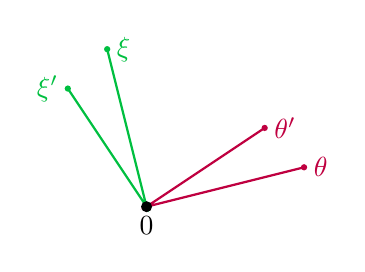
\begin{tikzpicture}
\draw[thick,green!75!blue](-1,3/2)--(0,0)--(-1/2,2);
\draw[thick,purple](2,1/2)--(0,0)--(3/2,1);
\draw(0,0)node[below]{$0$};
\draw[purple](2,1/2)node[right]{$\theta$};
\draw[purple](3/2,1)node[right]{$\theta^{\prime}$};
\draw[green!75!blue](-1/2,2)node[right]{$\xi$};
\draw[green!75!blue](-1,3/2)node[left]{$\xi^{\prime}$};
\fill[black](0,0)circle(0.07);
\fill[purple](2,1/2)circle(0.04);
\fill[purple](3/2,1)circle(0.04);
\fill[green!75!blue](-1/2,2)circle(0.04);
\fill[green!75!blue](-1,3/2)circle(0.04);
\end{tikzpicture}
\end{center}



}

\frame{\small 

\begin{Prop}[explicit formulae]\label{prop:exfdivhyperboloid}
%We have the following results for two hyperboloid distributions $p_{\theta}$ and $p_{\theta^{\prime}}$.\\
(i) (Kullback-Leibler) 
Let $f(u) = -\log u$.
Then, 
\begin{equation*}
D_f [p_{\theta}:p_{\theta^{\prime}}] 
= \log \left(\frac{|\theta|}{|\theta^{\prime}|}\right) - |\theta^{\prime}| + \frac{[\theta,\theta^{\prime}]}{[\theta,\theta]} + \frac{[\theta,\theta^{\prime}]}{|\theta|} -1.  
\end{equation*}

(ii) (squared Hellinger) 
Let $f(u) = (\sqrt{u} - 1)^2 / 2$. 
Then, 
\begin{equation*}
D_f [p_{\theta}: p_{\theta^{\prime}}] 
= 1 - \frac{2|\theta|^{1/2}|\theta^{\prime}|^{1/2} 
\exp\left(|\theta|/2 + |\theta^{\prime}|/2\right)}{ |\theta+\theta^{\prime}|  \exp\left(|\theta+\theta^{\prime}|/2\right)}.
\end{equation*}

(iii) (Neyman $\chi^2$)
Let $f(u) := (u-1)^2$. 
Assume that $2\theta^{\prime} - \theta \in \Theta_{\mathbb{L}^2}$. 
Then, 
\begin{equation*}
D_f [p_{\theta}: p_{\theta^{\prime}}] 
= \frac{|\theta^{\prime}|^2 \exp(2|\theta^{\prime}|)}{|\theta||2\theta^{\prime}-\theta|\exp(|\theta| + |2\theta^{\prime}-\theta|)} - 1. 
\end{equation*}
%corrected-1-16; 2023/04/30
\end{Prop}

This corresponds to Proposition \ref{prop:SHNC-Poincare} for Poincar\'e distributions. 

}

\frame{\frametitle{Correspondence}\small 

\begin{Prop}[Correspondence between the parameter spaces]\label{prop:corresp}
A bijection: 
\[ \Theta \longrightarrow \Theta_{\mathbb L}\] 
\[ \theta := (a,b,c) \mapsto \theta_{\mathbb L} := (a+c, a-c, 2b)  \]

By this map, \\
(i) For $\theta, \theta^{\prime} \in \Theta_{\mathbb H}$, 
\begin{equation*}\label{eq:corres-norm} 
|\theta_{\mathbb L}|^2 = \left[\theta_{\mathbb L},\theta_{\mathbb L}\right] = 4 |\theta|, \ |\theta^{\prime}_{\mathbb L}|^2 = \left[\theta^{\prime}_{\mathbb L},\theta^{\prime}_{\mathbb L}\right] = 4 |\theta^{\prime}|, \ \left[\theta_{\mathbb L},\theta^{\prime}_{\mathbb L}\right] = 2 |\theta| \textup{tr}(\theta^{\prime} \theta^{-1}).
\end{equation*}
(ii) For every $f$ and $\theta, \theta^{\prime} \in \mathbb{H}$, 
\begin{equation*}\label{eq:corres}
D_f^{\mathbb L}\left[p_{\theta_{\mathbb L}}:p_{\theta^{\prime}_{\mathbb L}}\right] = D_f^{\mathbb H}\left[p_{\theta}:p_{\theta^{\prime}}\right].
\end{equation*}
\end{Prop}

There is also a correspondence between the sample spaces, which is compatible with the above one. 





}

\frame{\frametitle{Some references}\small

Barbaresco, F.: {\it Lie group machine learning and Gibbs density on Poincar\'e unit disk from Souriau Lie groups thermodynamics and SU(1,1) coadjoint orbits.} In: International Conference on GSI. pp. 157-170. Springer (2019)

\vspace{0.5pc}

Barndorff-Nielsen, O.: {\it Hyperbolic distributions and distributions on hyperbolae}. Scandinavian Journal of Statistics 5, 151-157 (1978)

\vspace{0.5pc}


Eaton, M.L.: {\it Group invariance applications in statistics}. Hayward, CA: Institute of Mathematical Statistics; Alexandria, VA: American Statistical Association (1989)

\vspace{0.5pc}

Jensen, J.L.: {\it On the hyperboloid distribution}. Scandinavian Journal of Statistics 8, pp. 193-206 (1981)


\vspace{0.5pc}

Sarkar, R.: {\it Low distortion {D}elaunay embedding of trees in hyperbolic plane}, Graph drawing, LNCS 7034, 355-366, (2012)

\vspace{0.5pc}

Tojo, K., Yoshino, T.: {\it An exponential family on the upper half plane and its conjugate prior}. In: Workshop on Joint Structures and Common Foundations of Statistical Physics, Information Geometry and Inference for Learning. pp. 84-95. Springer (2020)

}





\end{document}


Example of $f$-divergences: 
\begin{itemize}
\item Kullback-Leibler: $f(u) = -\log u$
\item squared Hellinger: $f(u) = (\sqrt{u} - 1)^2 / 2$
\item Neyman $\chi^2$: $f(u) := (u-1)^2$ 
\item total variation: $f(u)=|u-1|$
\end{itemize}




@incollection {MR2928298,
    AUTHOR = {Sarkar, Rik},
     TITLE = {Low distortion {D}elaunay embedding of trees in hyperbolic
              plane},
 BOOKTITLE = {Graph drawing},
    SERIES = {Lecture Notes in Comput. Sci.},
    VOLUME = {7034},
     PAGES = {355--366},
 PUBLISHER = {Springer, Heidelberg},
      YEAR = {2012},
      ISBN = {978-3-642-25877-0},
   MRCLASS = {05C62 (51M10 52A55)},
  MRNUMBER = {2928298},
       DOI = {10.1007/978-3-642-25878-7\_34},
       URL = {https://doi.org/10.1007/978-3-642-25878-7_34},
}











